\documentclass[format=acmlarge]{acmart}

\usepackage{amsmath}
\DeclareMathOperator*{\argmax}{argmax}

\usepackage{hyperref}

\setcopyright{rightsretained}
\copyrightyear{2017}

\begin{document}
\title{Using neural network techniques to correlate past and future large-cap stock returns}

\author{Kenneth Allen}
\affiliation{%
  \institution{Armstrong State University}
  \department{Department of Computer Science \& Information Technology}
  \city{Savannah}
  \state{GA}
  \postcode{31419}
  \country{United States of America}}
\email{ka3878@stu.armstrong.edu}

\author{Jeffrey Young}
\affiliation{%
  \institution{Armstrong State University}
  \department{Department of Computer Science \& Information Technology}
  \city{Savannah}
  \state{GA}
  \postcode{31419}
  \country{United States of America}}
\email{jy8672@stu.armstrong.edu}

\begin{abstract}
Quantitative analysis of the stock market to predict future behavior has long been a very active area of study with clear applicability, both for profit-seeking and informing macroeconomic policy.  We apply support neural network techniques to show that simple daily total return data can be shown to be correlated with future performance.  Although our method is not immediately applicable for predicting beyond the current moment in time, it demonstrates that the potential for such models does exist.
\end{abstract}

\keywords{Machine learning, Neural networks, Neuroph, Stock prediction, S\&P 500}

\maketitle

\section{Backgound}
\begin{table}
  \caption{Historical S\&P predictor accuracy.}
  \label{tab:one}
  \begin{tabular}{l|l}
    Na\"{i}ve Bayesian & 60.38\%\\
    Linear SVM & 59.79\%\\
    RBF SVM & 62.51\%\\
    Polynomial SVM & 59.43\%\\
    Neural Network & 65.08\%\\
  \end{tabular}
\end{table}

Predicting movement of the stock is a longtime attractive topic.  The purpose of this research venture was to explore the usefulness of S\&P 500 data in relation to the use of machine learning methodology as a predictive model. The S\&P 500 Index is a free float-adjusted market capitalization-weighted stock market index in the United States. It is used to record and monitor daily changes of the largest companies of the American stock market and is the main indicator of the overall market performance in the United States.  Historically, many methods of S\&P 500 analysis have been implemented with varying results but, overall, three analysis types have been explored most often: Na\"{i}ve Bayesian, Support Vector Machines, and Neural Networks.  Table 1 gives some values for the success of historical efforts.

\subsection{Feature Selection}
Feature analysis for all three common types of S\&P 500 predicates have been similar.  The most common features extracted from S\&P 500 data have been daily returns, NASDAQ daily return, S\&P 500 momentum, and S\&P 500 rate-of-change.  For this project, we used daily total returns.

Define $c(t)$ as the weighted average closing price of all stocks in the index for day $t$.
\begin{itemize}
  \item S\&P 500 daily return: $\frac{c(t) - c(t-1)}{c(t-1)}$.
  \item NASDAQ daily return: as above, but with weights and stocks from the NASDAQ market.
  \item S\&P 500 momentum ($n = 4$): $\frac{c(t) - c(t-4)}{c(t-4)}$.
  \item S\&P 500 rate-of-change ($n = 4$): $\frac{c(t)}{c(t-4)}$.
  \item S\&P 500 momentum ($n = 3$): $\frac{c(t) - c(t-3)}{c(t-3)}$.
  \item S\&P 500 rate-of-change ($n = 3$): $\frac{c(t)}{c(t-3)}$.
\end{itemize}

\section{Data Processing}
\subsection{Data}
The economics department of Armstrong State University has a dataset spanning over 16 years of daily total returns for each stock listed in the Standard \& Poor's 500 Index, which consists of 505 stocks from 500 of the largest companies in the world, measured by total market capitalization.  We were given limited access to this data to perform the experiments for this project.  The data takes the form of dated percentage daily total returns and occupies about 23.8 mibibytes (25 million bytes).

For each test, 10\% of the data was randomly removed and used as a test set while the remaining 90\% was used as a training set.

\subsection{Training Labels}
Labels for this undertaking were calculated from the excluded data from the test period, which was chosen as the final year of the data:  March 22, 2016, to March 21, 2017.  Each stock was labeled with whether its total return exceeded that of the S\&P 500 index during that period.

\subsection{Classifier}
\begin{figure}
  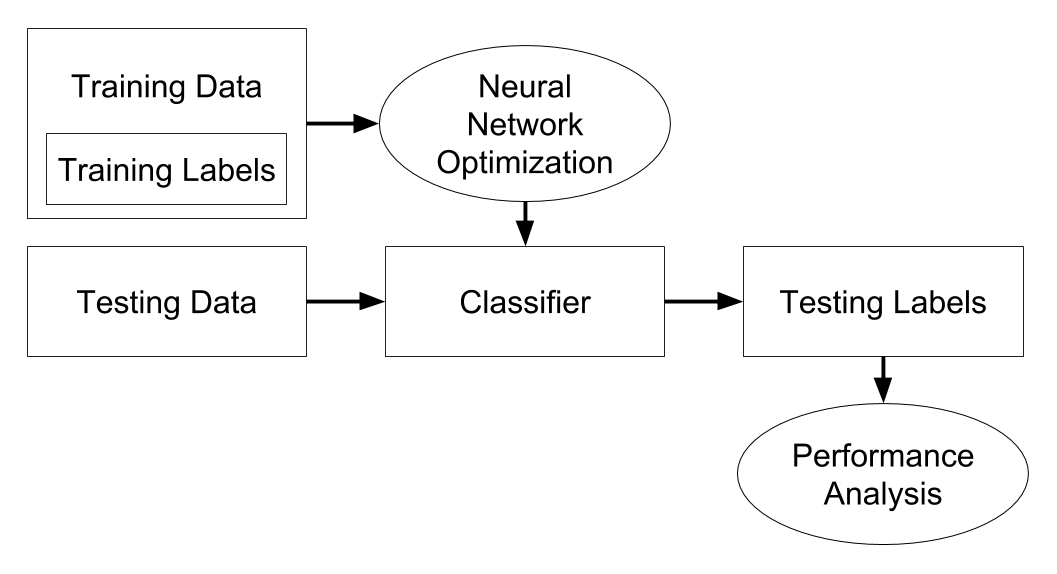
\includegraphics{block-diagram}
  \caption{Block diagram of classifier system.}
  \label{fig:one}
\end{figure}

Our system uses the Neuroph library to implement neural network training and classification.  It interacts with its programmatic Java API to add features like statistics tracking and training models with different sensitivities.  We tested different numbers of layers and layer sizes, and achieved our best results with a single hidden layer of 30 neurons, connected to an input layer of 4075 features and an output layer of a single neuron.  Parameters like maximum error, maximum optimization passes, and starting weight randomization were taken from values recommended by the library authors.

\subsection{Prediction}
Prediction quality was measured with a bevy of statistics.  Accuracy is simple to calculate ($\frac{\textrm{correct classifications}}{\textrm{tested elements}}$).

For binary criteria, more informative values can be generated.  Use $\mathit{TP}$, $\mathit{FP}$, $\mathit{FN}$, and $\mathit{TN}$, to represent true positives, false positives, false negatives, and true negatives, respectively.  Especially important are true positive rate ($\mathit{TPR} = \frac{\mathit{TP}}{\mathit{TP} + \mathit{FN}}$), true negative rate ($\mathit{TNR} = \frac{\mathit{TN}}{\mathit{FP} + \mathit{TN}}$), positive predictive value ($\mathit{PPV} = \frac{\mathit{TP}}{\mathit{TP} + \mathit{FP}}$), and negative predictive value ($\mathit{NPV} = \frac{\mathit{TN}}{\mathit{FN} + \mathit{TN}}$).

The $F_1$ score is calculated as the harmonic mean of $\mathit{TPR}$ and $\mathit{PPV}$:

$$F_1 = \frac{2}{\frac{1}{\mathit{TPR}} + \frac{1}{\mathit{PPV}}}$$

\subsection{Receiver Operating Characteristic}
\begin{figure}
  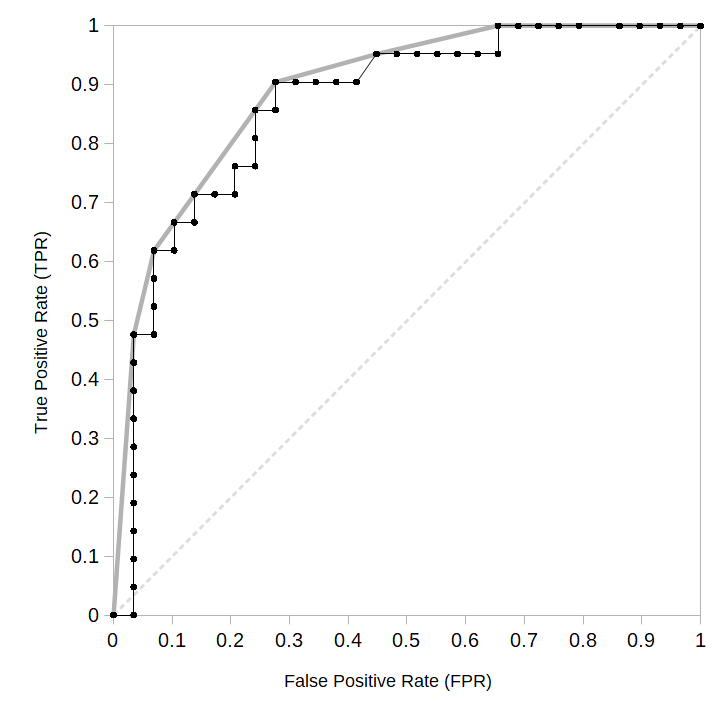
\includegraphics{interpolated-roc}
  \caption{Receiver Operating Characteristic with interpolated convex hull.}
  \label{fig:two}
\end{figure}

By tuning our sensitivity parameter, we can adjust our tradeoff between excluding false negatives and including false positives.  Plotted on a graph, we see our Receive Operating Characteristic, or ROC.  The area under these points creates our ``AUC'' statistic, or area-under-the-curve (the `curve' being the black line in Fig. 2).  $0.5$ is the AUC of a totally random classifier (like the dashed line in Fig. 2), and $1$ is only achievable with no mistakes.  AUC is more representative than simple accuracy because it takes into account the spectrum of configurations for the classifier's sensitivity.

We can trivially interpolate between these points by imagining a series of classifiers that randomly choose with a certain probability to defer to one of two of our classifiers, creating a `line' of these between those two points.  If we choose to apply this technique to the convex hull of our points, we get an improved curve that interpolates between our best results and represents the best the classifier is capable of (the solid gray line on Fig. 2).  We calculate the area under this curve as our ``interpolated AUC''.

\section{Results and Performance}

\begin{table}
  \caption{Classifier results.}
  \label{tab:two}
  \begin{tabular}{l|l}
    ($\textrm{sensitivity} = 0.5$) Accuracy & 0.800\\
    ($\textrm{sensitivity} = 0.5$) PPV & 0.704\\
    ($\textrm{sensitivity} = 0.5$) NPV & 0.913\\
    ($\textrm{sensitivity} = 0.5$) $F_1$ score (positive condition) & 0.792\\
    ($\textrm{sensitivity} = 0.5$) $F_1$ score (negative condition) & 0.808\\
    ($\textrm{sensitivity} = 0.5$) simulated return & 35.1\%\\
    ROC AUC & 0.865\\
    ROC AUC (interpolated) & 0.892\\
  \end{tabular}
\end{table}

Table 2 gives statistics for one run of the classifier, with sensitivity set to $0.5$.  The classifier shows a clear bias for being better at rejecting underperforming stocks than determining overperforming ones.  We simulate a return value for the test period by determining what the return would have been for an investment split equally between the classifier's chosen stocks, and it significantly outperforms a simple index fund over the same period.

Our AUC values are very encouraging, suggesting that this classifier could be the basis of a powerful tool to evaluate stock likenesses for a variety of desired sensitivities.

\begin{table}
  \caption{Example classification of test set ($\textrm{sensitivity} = 0.5$).}
  \label{tab:three}
  \begin{tabular}{ll|ll|ll}
    JWN & -25.3\% & VIAB & 9.7\% & BDX* & 21.7\%\\
    CVS & -21.7\% & STZ & 10.6\% & \textbf{CTXS} & 30.9\%\\
    AN & -10.1\% & \textbf{AKAM}* & 12.0\% & \textbf{JEC} & 31.1\%\\
    COG & -7.1\% & \textbf{GWW}* & 12.6\% & \textbf{UNP} & 31.8\%\\
    MOS & -1.8\% & ADS & 12.8\% & \textbf{AAPL} & 34.7\%\\
    ORLY & -1.5\% & TMO & 12.8\% & \textbf{KLAC} & 36.1\%\\
    O & 0.1\% & TDC & 15.0\% & \textbf{DGX} & 43.6\%\\
    \textbf{GE}* & 0.3\% & AET & 16.3\% & \textbf{ROK} & 45.1\%\\
    K & 0.8\% & DTE & 16.6\% & \textbf{CMI} & 47.3\%\\
    \textbf{APA}* & 1.5\% & PNW & 17.3\% & \textbf{TXN} & 47.8\%\\
    \textbf{FLR}* & 2.4\% & \textbf{FISV}* & 17.3\% & \textbf{ULTA} & 48.2\%\\
    SO & 3.2\% & CVX & 17.5\% & \textbf{FITB} & 53.5\%\\
    \textbf{DNB}* & 6.7\% & \textit{S\&P 500} & 17.5\% & \textbf{WDC} & 59.9\%\\
    NWSA & 7.4\% & \textbf{WAT} & 17.9\% & \textbf{PFG} & 63.5\%\\
    DPS & 7.5\% & \textbf{WFC} & 19.7\% & \textbf{CSX} & 79.8\%\\
    CL & 8.8\% & \textbf{HOLX} & 20.5\% & \textbf{RF} & 81.1\%\\
    \textbf{JNPR}* & 9.0\% & KHC* & 20.7\% & \textbf{URI} & 94.0\%\\
  \end{tabular}
\end{table}

Table 3 gives the specific results from the network configured with a sensitivity of $0.5$.  The stocks are sorted by increasing return during the test period, and those that were predicted to outperform the S\&P 500 index have their tickers bolded.  The false positives (GE, APA, FLR, DNB, JNRP, AKAM, GWW, and FISV) and false negatives (KHC and BDX) are marked with asterisks.  The index itself is italicized in approximately the middle of the list, where one would expect it.

\section{Discussion}
\subsection{Applications}
Although we used `foreknowledge' of the test period to train our model, these results do demonstrate that stocks that will outperform the market in the future could have similarities in their past performance that machine learning techniques can discuss.  One application of this would be for someone with expert knowledge or insider information to label a training set of stocks.  Neural network optimization would create a model that could evaluate whether other stocks are `like' the expert's picks.  Another application could be to time-shift data and see if there are recognizable patterns in daily returns that repeat over intervals, which could potentially be projected into the future.

\subsection{Conclusion}
Machine learning techniques can be used to distinguish effectively between large-cap stocks that will and will not outperform the market over a specific period of time.  Neural networks are well-suited to this task because of how they are able to detect subtle correlations even among thousands of variables.  Although our model was constructed using foreknowledge of stocks' performance, other, less absolute methods could be used to label training data for the same or similar purposes.

\section{Works Cited}
\begin{itemize}
  \item \textit{Forecasting S\&P 500 Stock Index Using Statistical Learning Models}. Available from: https://www.researchgate.net/publication/311502789\_Forecasting\_SP\_500\_Stock\_Index\_Using\_Statistical\_Learning\_Models [accessed Dec 04 2017].
  \item Lin, H. (n.d.). \textit{Feature Investigation for Stock market Prediction}. Retrieved from http://cs229.stanford.edu/proj2013/Lin-Feature\%20Investigation\%20for\%20Stock\%20Market\%20Prediction.pdf
  \item Akita, R., Yoshihara, A., Matsubara, T., \& Uehara, K. (2016). Deep learning for stock prediction using numerical and textual information. \textit{2016 IEEE/ACIS 15th International Conference on Computer and Information Science (ICIS)}. doi:10.1109/icis.2016.7550882
\end{itemize}

\end{document}